\documentclass[PICOReport.tex]{subfiles}

%\newcolumntype{L}[1]{>{\raggedright\let\newline\\\arraybackslash\hspace{0pt}}m{#1}}
%\newcolumntype{K}[1]{>{\raggedright\centering\arraybackslash}m{#1}}

\begin{document}

Having flown two space missions (WMAP and \planck ) and fielded numerous sub-orbital experiments to measure polarization, the mm/sub-mm wavelength community has gained extensive experience with systematic uncertainties that occur in various experimental configurations. 
A rich literature investigates the types of systematic errors due to the environment, the instrumentation, observation strategies, and data analysis that could confound polarization measurements by creating a bias or an increased variance \cite{hu03,shimon2008,yadav2010,Griffiths2014,LFI_systematics,Kaplan2002,Miller2009,Pagano2009}. Teams have used the accumulated experience to incorporate technological solutions during the design phase, and to optimize data analysis techniques to identify and compensate for systematic errors. 
%As a consequence, all of the cosmological results reported to date are noise, not systematic uncertainty limited. In several cases systematic effects have been identified in the data, but then suppressed to levels below the noise. 

Just as requirements on signal separation (\S~\ref{sec:signal_separation}) are determined by the need to reach the faintest inflationary signal so are the requirements on control of systematic uncertainties. Since an inflationary $BB$ power spectrum with $r = 5 \times 10^{-4}$ has a peak signal level of 7~nK, systematic effects need to be controlled to a level of $\sim$1~nK. It has long been recognized that exquisite control of systematic uncertainties will be required from any experiment attempting to reach levels of $r \lesssim 1\times 10^{-3}$, and it is widely accepted that the stability provided aboard a space platform makes it best suited to control systematic uncertainties compared to other platforms. This is one of the most compelling reasons to observe from space.  As WMAP and \planck~ demonstrated, an L2 orbit offers excellent stability, as well as flexibility in the choice of scan strategy.  PICO takes advantage of an L2 orbit, using a rotating spacecraft (at 1~rpm) whose spin axis precesses with a 10~hour period, thus scanning the sky in a way that is crosslinked on many time scales and at many angles, without interference from the Sun, Earth, or Moon; this reduces the effects of low frequency noise without the need for additional internal-to-the-instrument mechanical modulation. The redundancy of observations allows the checking of consistency of results and an improved ability to calibrate and to correct systematic errors in post-processing analysis.

\comor{now here}
% redundancy: 13,000 independent q,u,i maps; 10 independent surveys maps of the sky
%We expect the following paradigm to continue: if a systematic effect is large enough to exist above the noise level, it can be characterized and suppressed. 


%A rich literature investigates the types of systematic errors due to the environment, the instrumentation, observation strategies, and data analysis that could confound polarization measurements by creating a bias or an increased variance \cite{hu03,shimon2008,yadav2010}. Every measurement to date has  reached a systematic error limit, 

%\comor{what do you mean?} 
and many sophisticated techniques have been advanced to mitigate systematics, finding both new technological solutions and new analysis techniques. As an example, BICEP systematics limited it to r=0.1\cite{Takahashi2010} while through additional effort within the program, BICEP2 achieved a systematics limit of r=6$\times$10$^{-3}$\cite{BICEP2_III}). In the near term, the ground-based and suborbital CMB community will continue to develop new techniques in handling systematics, particularly in developing the CMB-S4 project.

%\comor{what does paragraph try to say?}
All prior on-orbit measurements of CMB polarization were limited by systematic errors until an in-depth study of the systematics was performed allowing a post-processing data analysis to suppress them \cite{Bennett13,planck2016_xlvi,Planck2018_I}. Particularly we note figure 3 of Ref.\cite{Planck2018_I} which quantifies \planck's systematic error limits on the polarization power spectral measurements. Recently studied space missions, such as EPIC-IM, LiteBird and  \core, have placed systematic error mitigation at the forefront of the case for their mission and have developed tools and strategies for estimating and mitigating these\cite{hazumi2012,wallis2017,Natoli2018}.

Systematic effects are coupled with the spacecraft scan strategy, and the details of the data analysis pipeline. Thus, end-to-end simulation of the experiment is an essential tool, including realistic instabilities and non-idealities of the spacecraft, telescope, and instrument, as well as folding in data post-processing techniques used to mitigate the systematic effects.    

\subsubsection{List of Systematics}
\label{sec:systematics_list}

The systematic errors faced by PICO can be categorized into three broad categories: 
1) Coupling of the intensity into the polarization signal; 2) stability; and 3) straylight. These are listed in Table \ref{tbl:SystematicsList2col} and were prioritized for further study using a risk factor incorporating the working group's assessment of how mission-limiting the effect is, how well these effects are understood by the community and whether mitigation techniques exist.  

The three highest risk systematic errors were studied further and are discussed in subsections below.  The PICO team used 
 simulation and analysis tools developed for \planck~\cite{plank2015_xii_focalplane} and \core, adapting them for PICO.

%We note that many of the systematics could be mitigated further through the use of polarization modulation such as a half-wave plate or a variable phase delay modulator.  
%For the purposes of the cost constraints of PICO, we investigated mitigation techniques that do not require a modulator.  

\begin{table}[h!]
\hspace{-0.1in}
\parbox{3.5in}{
\centering
\scriptsize
 \begin{tabular}{p{3.3cm} p{0.5cm} p{1.4cm} p{1.7cm}}
 \hline
\textbf{Name} & \textbf{Risk}&\textbf{Effect} \\
 \hline
\textbf{Leakage}& &\\
Polarization angle calibration\dotfill& 
5&
$E{\to}B$ &
Sect.~\ref{sec:angle}.
\\
 Bandpass mismatch\dotfill&
 4& 
$T{\to}$P, $E{\to}B$  
   \\
Beam mismatch\dotfill& 
4&
$T{\to}$P, $E{\to}B$
& Sect.~\ref{sec:angle}
\\
Time response accuracy and stability\dotfill&
4&
$T{\to}$P, $E{\to}B$
\\
Readout cross-talk\dotfill& 
4&
spurious P
\\
Chromatic beam shape\dotfill&
4&
spurious P
\\

Gain mismatch\dotfill&
3&
$T{\to}$P   
\\


Cross-polarization\dotfill&
3&
$E{\to}B$
\\
\hline 
\textbf{Stability} & & \\
Gain stability\dotfill& 
5&
$T{\to}$P, $E{\to} B$
& 
Sect.~\ref{sec:gain}
\\
Pointing jitter\dotfill&
3&
$T{\to}$P, $E{\to}B$
\\

\hline
\textbf{Straylight}& & \\
Far sidelobes\dotfill& 
5&
spurious P
&
Sect.~\ref{sec:fsl}.\\
 \hline
\textbf{Other} \\
Residual correlated noise (1/f, cosmic ray hits)\dotfill&
3 &
increased variance
\\
\hline
 \end{tabular}
}
\hspace{-0.0in}
\parbox{3.1in}{
\caption{\captiontext
Enumeration of potential systematic errors anticipated in \pico's measurements together with their assessed risk level, 
%for affecting measurement of the inflationary signal, 
their effect on the measurements, and, in few cases, subsections with further discussion. The symbol $T \rightarrow P$ denotes coupling of the intensity (=temperature) signal into polarization; similar meaning holds for the $E$ and $B$ modes.  Risk level rises with value. Level 5 indicates a highly significant, design-driving effect; it may have limited past measurements, and/or isn't well understood.  Level 4 indicates an effect that is either known to be large but is understood reasonably well, or a smaller effect that requires precise modeling.  Level 3 indicates that we expect the effect to be small, but it is not sufficiently well understood and detailed modeling will be done during Phase A study. We used simulations to investigate effects with risk level 5.
\label{tbl:SystematicsList2col} }}
\hspace{-0.0in}
\end{table}


\subsubsection{Absolute Polarization Angle Calibration}
\label{sec:angle}

The measured CMB polarization can be rotated due to (1) a birefringent primordial Universe, or a Faraday rotation
due a primordial magnetic field \citep{Pogosian+2018}; (2) birefringent
foregrounds, or interaction with the Galactic magnetic field;
(3) systematic effects in the instrument, and in particular an error in
the direction of polarization measured by each detector.  
While the first two sources create a rotation that may depend on scale,
position and/or frequency, the latter depends mainly on
the detector itself. 

A rotation {\prang} of the direction of polarization mixes the $Q$ and $U$ Stokes parameters via
$Q\pm iU \longrightarrow e^{\mp i 2 \prang} (Q\pm iU)$
and thus mixes the power spectra and their correlations, as illustrated in Fig.~\ref{fig:rot_bb_tb_eb}.


%------------------------------------------------------------------------------------------

The most recent constraints on cosmological birefringence \citep{Planck2016_XLIX} were limited by uncertainties on the detector orientations.  In \planck, the detectors were characterized pre-launch to $\pm 0.9^\circ$ (rel.) $\pm 0.3^\circ$ (abs.) \citep{Rosset+2010}. For \pico, the relative rotation of the detectors will be measured to a few $0.1\arcmin$ using the CMB, but the overall rotation is unlikely to be known pre-launch to better than \planck.  Known polarized sources, such as the Crab Nebula, are not characterized well enough independently to serve as calibrators; \citet{Aumont+2018} show that the current uncertainty of $0.33^\circ$ on the Crab polarization orientation, limits a $B$-mode measurement to $r \sim 0.01$, far from \pico's target.

%Figures \ref{fig:rot_sens_0} and \ref{fig:rot_sens_2} show how the measurement of $r$ by \pico\ is degraded because of an overall rotation of polarization, and how $TB$ and $EB$ can be used to monitor this rotation, assuming that the only source of polarization rotation is instrumental.
%These results are obtained assuming the spectra to have a Gaussian likelihood, with a variance $\propto 1/\fsky$, and ignoring the foreground contributions.

In the absence of other systematics and foregrounds, a polarization rotation error $\alpha$ of $10\arcmin$ degrades 
the uncertainty of $r$ by 30\%, while $EB$, $TB$, and $BB$ spectra can measure a rotation $\alpha$ at 3$\sigma$ when $\alpha = 0.07, 0.2$  and $0.9\arcmin$, respectively,
 on perfectly delensed maps, and $0.25, 0.9$, and $4.5\arcmin$ on raw maps.

In principle, the technique of using the $TB$ and $EB$ spectra can measure a global polarization rotation error at levels (around $0.1 \arcmin$) below those affecting $r$ measurements in $BB$ ($> 1 \arcmin$).  However, a future mission should simulate additional aspects of this issue, such as delensing, the interaction with foregrounds, and $1/f$ noise in simulating and assessing the impact of an angle-calibration error.

\subsubsection{Gain Stability}
\label{sec:gain_stability}


Photometric calibration is the process of converting the raw output of each detector to physical units via the characterization of the `gain factor' $G(t)$, which is a function of time. Statistical or systematic errors in the determination of $G$ translate to increased uncertainties, or biased results, respectively.  We investigated whether the anticipated error on $G$ is adequate for PICO's requirements on measuring the faint inflationary signal.  

The inflationary signal will be extracted from data in the primary CMB bands between $\sim$60 and $\sim$300~GHz. Detectors in these bands will be calibrated using measurements of the CMB dipole, a signal that will be measured once per minute as the telescope scans the sky (\S~\ref{sec:survey_design}).  We evaluated the combined impact of the scan strategy and white- and 1/f-noise in the estimation of $G(t)$.\footnote{We use software tools developed for and validated in the context of analysis of the \planck/LFI data.} The simulation included signals from the anisotropy of the CMB, including the dipole, but due to limited resources it did not include Galactic foregrounds. Full details of the simulation pipeline are available in the PICO website~\citep{pico_web}. Fig.~\ref{fig:rot_bb_tb_eb} demonstrates that the power spectrum due to error in $G(T)$ is much lower than the PICO requirement of $\sigma(r) = 1\times 10^{-4}$. 
\begin{figure}[thb]
\includegraphics[width=0.6\textwidth]{images/PICO_rotate_eb5_v1.\suffix} 
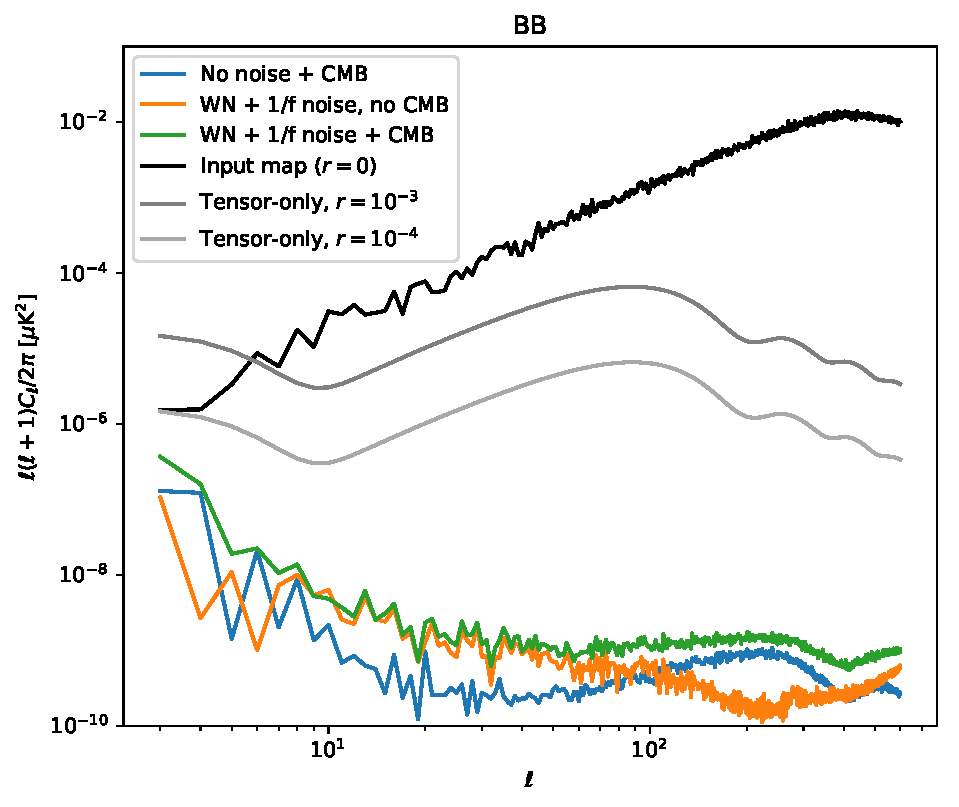
\includegraphics[width=0.35\textwidth]{images/calibration_spectrum_BB.pdf}
\caption{\captiontext
Left and center: Spurious power due to a rotation of the angle of polarization, assuming the \planck~2018 $\Lambda$CDM model \citep{Planck2018_VI} with $\tau=0.054$ and expected \pico\ noise performance, assuming removal of 85\% of the lensing power.  Right: residual power after removal of temporal gain drifts using the dipole.
\label{fig:rot_bb_tb_eb} }
\end{figure}

A more complete data-analysis pipeline would pair the calibration step with the component-separation step, following a schema similar to \planck/LFI's final data processing \cite{Planck2018_II}: the calibration code is followed by a component-separation analysis, and these two steps are iterated until the solution converges. 

%We simulated the time stream signals of four detectors over the duration of the mission, including PICO baseline noise levels, 1/f noise parameters, and the scan strategy. We solved (\S~\ref{sec:??}) \comor{where?}. We fit the  an end-to-end simulation using

%instrument and the CORE mission proposal. The quality of the estimate depends on the noise level of the receivers, but also on the details of the scanning strategy.  To analyze the impact of calibration uncertainties on PICO, we performed  the following analysis. Firstly, we simulated the observation of the sky, assuming four receivers, the nominal scanning strategy, and $1/f$ noise. The simulated sky contained CMB anisotropies, plus the CMB dipole. Then we ran the calibration code to fit the dipole against the raw data simulated during the first step. We again simulated the observation of the sky, this time using the values of $G$ computed during the second step, which contain errors due to the presence of noise and the CMB signal.

%Results of the simulation (neglecting foregrounds) are shown as power spectrum residuals in Fig.~\ref{fig:rot_bb_tb_eb}. We estimate the gain fluctuations to better than 10$^{-4}$ when solving for the gain every 40 hours (4 precession periods). The scanning strategy employed by PICO allows for a much better calibration than was possible for \planck, thanks to the much faster precession.

\subsubsection{Far-Sidelobe Pickup}
\label{sec:fsl}
%The main beam (within a few degrees of the axis of beam response) in a CMB mission can be measured to high precision using the planets .  
Measurement of each detector's response to signals off axis, which tends to be weak (--80dB less than the peak response) but spread over a very large solid angle, is difficult to do pre-launch, and may not even be done accurately after launch.  Nonetheless, this far sidelobe can couple bright Galactic signals from many tens of degrees off-axis and confuse it with polarized signal from the CMB off the Galactic plane.    To evaluate this systematic error, GRASP software\footnote{https://www.ticra.com} was used to compute the \pico\ telescope's response over the full sky.  The computed full-sky beams showed features peaking at about -80\,dB of the on-axis beam.   
This full-sky beam was convolved with a polarized Galactic signal and a one-year \pico\ mission scan using the simulation pipeline; this preliminarily shows that the far sidelobe pickup must be reduced by 90\%  to keep the sidelobe signal from appreciably increasing the variance on the B-mode power measurement.
This reduction can be achieved by adjusting the instrument design or by modeling, measuring, and removing the sidelobe pickup during data analysis.

\subsubsection{Key Findings}
\label{sec:systematics_key}

Properly modeling, engineering for, and controlling the effects of systematic errors in a
next-generation CMB probe is critical.  As of today, we conclude that there is a clear path to demonstrate that state-of-the-art technology and data processing can take advantage of the L2 environment and control systematic errors to a level that enables the science goals of PICO. In particular we note the following points:
\begin{itemize}
\item The raw sensitivity of the instrument should include enough margin
that data subsets can independently achieve the science goals.
This allows testing of the results in the data analysis and additional
data cuts, if needed.
\item For PICO mission, a physical optics model of the telescope should be developed, enabling full-sky beam calculations, which should be validated as much as possible on the ground.  This will be needed to characterize and remove far-sidelobe pickup seen during the mission. 
\item NASA's support of ground-based and suborbital CMB missions will mitigate risk to a future space mission such as PICO by continuing to develop analysis techniques and technology for the reduction of systematic errors.

\item In the PICO mission's phase A, a complete end-to-end system-level
simulation software facility should be developed to assist the team in setting 
requirements and conducting trade-offs between subsystem requirements while
realistically accounting for post-processing mitigation.  Any future
CMB mission is likely to have similar orbit  
and scan characteristics to those of PICO, thus there is an opportunity for NASA and
the CMB community to invest in further development of this capability now.
\item Low frequency excess noise (also called 1/f noise) should be studied in detail as part of a simulation effort to set detailed detector and systems level requirements.  The systematics simulations performed here show that PICO's science goals can be achieved with no additional modulation and assuming current state-of-the-art levels of low frequency noise (a total knee frequency of 20 mHz) based on demonstrated TES performance, and system-level residuals achieved by \planck.
\end{itemize}

\end{document}

